\begin{figure}[!tbh]
  \resizebox{\linewidth}{!}{
    \centering
    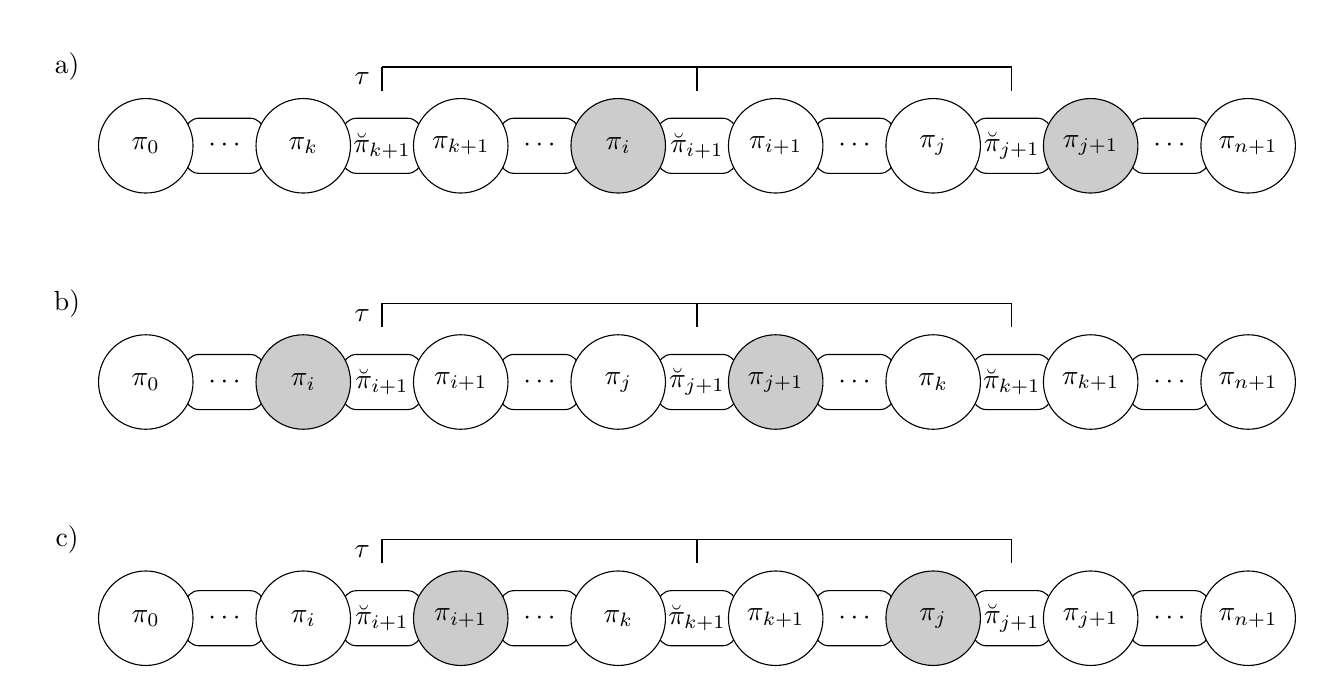
\begin{tikzpicture}
      %%%%% a)

      \node[draw=none,fill=none, minimum height=1cm, minimum width=1cm] at (-3.0, -2.0) {a)};

      % intergenic regions
      \node[rectangle,draw,fill=white!20, minimum height=.7cm, minimum width=1cm, rounded corners=5pt] at (-1.0, -3.0) {$\cdots$};
      \node[rectangle,draw,fill=white!20, minimum height=.7cm, minimum width=1cm, rounded corners=5pt] at (1.0, -3.0) {$\breve\pi_{k+1}$};
      \node[rectangle,draw,fill=white!20, minimum height=.7cm, minimum width=1cm, rounded corners=5pt] at (3.0, -3.0) {$\cdots$};
      \node[rectangle,draw,fill=white!20, minimum height=.7cm, minimum width=1cm, rounded corners=5pt] at (5.0, -3.0) {$\breve\pi_{i+1}$};
      \node[rectangle,draw,fill=white!20, minimum height=.7cm, minimum width=1cm, rounded corners=5pt] at (7.0, -3.0) {$\cdots$};
      \node[rectangle,draw,fill=white!20, minimum height=.7cm, minimum width=1cm, rounded corners=5pt] at (9.0, -3.0) {$\breve\pi_{j+1}$};
      \node[rectangle,draw,fill=white!20, minimum height=.7cm, minimum width=1cm, rounded corners=5pt] at (11.0, -3.0) {$\cdots$};

      % genes
      \node[draw, circle, minimum height=1.2cm, minimum width=1.2cm, fill=white!20] at ({(2*0 - 2)}, -3.0) {$\pi_{0}$};
      \node[draw, circle, minimum height=1.2cm, minimum width=1.2cm, fill=white!20] at ({(2*1 - 2)}, -3.0) {$\pi_{k}$};
      \node[draw, circle, minimum height=1.2cm, minimum width=1.2cm, fill=white!20] at ({(2*2 - 2)}, -3.0) {$\pi_{k+1}$};
      \node[draw, circle, minimum height=1.2cm, minimum width=1.2cm, fill=black!20] at ({(2*3 - 2)}, -3.0) {$\pi_{i}$};
      \node[draw, circle, minimum height=1.2cm, minimum width=1.2cm, fill=white!20] at ({(2*4 - 2)}, -3.0) {$\pi_{i+1}$};
      \node[draw, circle, minimum height=1.2cm, minimum width=1.2cm, fill=white!20] at ({(2*5 - 2)}, -3.0) {$\pi_{j}$};
      \node[draw, circle, minimum height=1.2cm, minimum width=1.2cm, fill=black!20] at ({(2*6 - 2)}, -3.0) {$\pi_{j+1}$};
      \node[draw, circle, minimum height=1.2cm, minimum width=1.2cm, fill=white!20] at ({(2*7 - 2)}, -3.0) {$\pi_{n+1}$};

      % indexes
      \draw (1.0, -2.3) -- (1.0, -2.0);
      \draw (5.0, -2.3) -- (5.0, -2.0);
      \draw (9.0, -2.3) -- (9.0, -2.0);
      \draw (1.0, -2.0) -- (9.0, -2.0);
      \node[draw=none,fill=none] at (0.75, -2.15) {$\tau$};

      %%%%% b)

      \node[draw=none,fill=none, minimum height=1cm, minimum width=1cm] at (-3.0, -5.0) {b)};

      % intergenic regions
      \node[rectangle,draw,fill=white!20, minimum height=.7cm, minimum width=1cm, rounded corners=5pt] at (-1.0, -6.0) {$\cdots$};
      \node[rectangle,draw,fill=white!20, minimum height=.7cm, minimum width=1cm, rounded corners=5pt] at (1.0, -6.0) {$\breve\pi_{i+1}$};
      \node[rectangle,draw,fill=white!20, minimum height=.7cm, minimum width=1cm, rounded corners=5pt] at (3.0, -6.0) {$\cdots$};
      \node[rectangle,draw,fill=white!20, minimum height=.7cm, minimum width=1cm, rounded corners=5pt] at (5.0, -6.0) {$\breve\pi_{j+1}$};
      \node[rectangle,draw,fill=white!20, minimum height=.7cm, minimum width=1cm, rounded corners=5pt] at (7.0, -6.0) {$\cdots$};
      \node[rectangle,draw,fill=white!20, minimum height=.7cm, minimum width=1cm, rounded corners=5pt] at (9.0, -6.0) {$\breve\pi_{k+1}$};
      \node[rectangle,draw,fill=white!20, minimum height=.7cm, minimum width=1cm, rounded corners=5pt] at (11.0, -6.0) {$\cdots$};

      % genes
      \node[draw, circle, minimum height=1.2cm, minimum width=1.2cm, fill=white!20] at ({(2*0 - 2)}, -6.0) {$\pi_{0}$};
      \node[draw, circle, minimum height=1.2cm, minimum width=1.2cm, fill=black!20] at ({(2*1 - 2)}, -6.0) {$\pi_{i}$};
      \node[draw, circle, minimum height=1.2cm, minimum width=1.2cm, fill=white!20] at ({(2*2 - 2)}, -6.0) {$\pi_{i+1}$};
      \node[draw, circle, minimum height=1.2cm, minimum width=1.2cm, fill=white!20] at ({(2*3 - 2)}, -6.0) {$\pi_{j}$};
      \node[draw, circle, minimum height=1.2cm, minimum width=1.2cm, fill=black!20] at ({(2*4 - 2)}, -6.0) {$\pi_{j+1}$};
      \node[draw, circle, minimum height=1.2cm, minimum width=1.2cm, fill=white!20] at ({(2*5 - 2)}, -6.0) {$\pi_{k}$};
      \node[draw, circle, minimum height=1.2cm, minimum width=1.2cm, fill=white!20] at ({(2*6 - 2)}, -6.0) {$\pi_{k+1}$};
      \node[draw, circle, minimum height=1.2cm, minimum width=1.2cm, fill=white!20] at ({(2*7 - 2)}, -6.0) {$\pi_{n+1}$};

      % indexes
      \draw (1.0, -5.3) -- (1.0, -5.0);
      \draw (5.0, -5.3) -- (5.0, -5.0);
      \draw (9.0, -5.3) -- (9.0, -5.0);
      \draw (1.0, -5.0) -- (9.0, -5.0);
      \node[draw=none,fill=none] at (0.75, -5.15) {$\tau$};

      %%%%% c)

      \node[draw=none,fill=none, minimum height=1cm, minimum width=1cm] at (-3.0, -8.0) {c)};

      % intergenic regions
      \node[rectangle,draw,fill=white!20, minimum height=.7cm, minimum width=1cm, rounded corners=5pt] at (-1.0, -9.0) {$\cdots$};
      \node[rectangle,draw,fill=white!20, minimum height=.7cm, minimum width=1cm, rounded corners=5pt] at (1.0, -9.0) {$\breve\pi_{i+1}$};
      \node[rectangle,draw,fill=white!20, minimum height=.7cm, minimum width=1cm, rounded corners=5pt] at (3.0, -9.0) {$\cdots$};
      \node[rectangle,draw,fill=white!20, minimum height=.7cm, minimum width=1cm, rounded corners=5pt] at (5.0, -9.0) {$\breve\pi_{k+1}$};
      \node[rectangle,draw,fill=white!20, minimum height=.7cm, minimum width=1cm, rounded corners=5pt] at (7.0, -9.0) {$\cdots$};
      \node[rectangle,draw,fill=white!20, minimum height=.7cm, minimum width=1cm, rounded corners=5pt] at (9.0, -9.0) {$\breve\pi_{j+1}$};
      \node[rectangle,draw,fill=white!20, minimum height=.7cm, minimum width=1cm, rounded corners=5pt] at (11.0, -9.0) {$\cdots$};

      % genes
      \node[draw, circle, minimum height=1.2cm, minimum width=1.2cm, fill=white!20] at ({(2*0 - 2)}, -9.0) {$\pi_{0}$};
      \node[draw, circle, minimum height=1.2cm, minimum width=1.2cm, fill=white!20] at ({(2*1 - 2)}, -9.0) {$\pi_{i}$};
      \node[draw, circle, minimum height=1.2cm, minimum width=1.2cm, fill=black!20] at ({(2*2 - 2)}, -9.0) {$\pi_{i+1}$};
      \node[draw, circle, minimum height=1.2cm, minimum width=1.2cm, fill=white!20] at ({(2*3 - 2)}, -9.0) {$\pi_{k}$};
      \node[draw, circle, minimum height=1.2cm, minimum width=1.2cm, fill=white!20] at ({(2*4 - 2)}, -9.0) {$\pi_{k+1}$};
      \node[draw, circle, minimum height=1.2cm, minimum width=1.2cm, fill=black!20] at ({(2*5 - 2)}, -9.0) {$\pi_{j}$};
      \node[draw, circle, minimum height=1.2cm, minimum width=1.2cm, fill=white!20] at ({(2*6 - 2)}, -9.0) {$\pi_{j+1}$};
      \node[draw, circle, minimum height=1.2cm, minimum width=1.2cm, fill=white!20] at ({(2*7 - 2)}, -9.0) {$\pi_{n+1}$};

      % indexes
      \draw (1.0, -8.3) -- (1.0, -8.0);
      \draw (5.0, -8.3) -- (5.0, -8.0);
      \draw (9.0, -8.3) -- (9.0, -8.0);
      \draw (1.0, -8.0) -- (9.0, -8.0);
      \node[draw=none,fill=none] at (0.75, -8.15) {$\tau$};
    \end{tikzpicture}
  }
  \caption[Exemplo de remoção de, pelo menos, um breakpoint tipo um após a aplicação de uma transposição $\tau$.]{Exemplo de remoção de, pelo menos, um breakpoint tipo um após a aplicação de uma transposição $\tau$.}
  \label{figure:WDJFPAXN}
\end{figure}